\documentclass{article}
% packages
\usepackage{amsmath,amssymb}
\usepackage{graphicx}
\usepackage{hyperref}

% directory of figures
%\graphicspath{ {figs} }

% latin bold lower
\newcommand{\ba}{\mathbf{a}}
\newcommand{\bc}{\mathbf{c}}
\newcommand{\be}{\mathbf{e}}
\newcommand{\bh}{\mathbf{h}}
\newcommand{\bp}{\mathbf{p}}
\newcommand{\bt}{\mathbf{t}}
\newcommand{\bs}{\mathbf{s}}
\newcommand{\bu}{\mathbf{u}}
\newcommand{\bv}{\mathbf{v}}
\newcommand{\bw}{\mathbf{w}}
\newcommand{\bx}{\mathbf{x}}
\newcommand{\by}{\mathbf{y}}
\newcommand{\bz}{\mathbf{z}}
\newcommand{\bm}{\mathbf{m}}

% latin bold upper
\newcommand{\bA}{\mathbf{A}}
\newcommand{\bB}{\mathbf{B}}
\newcommand{\bC}{\mathbf{C}}
\newcommand{\bI}{\mathbf{I}}
\newcommand{\bJ}{\mathbf{J}}
\newcommand{\bL}{\mathbf{L}}
\newcommand{\bM}{\mathbf{M}}
\newcommand{\bP}{\mathbf{P}}
\newcommand{\bQ}{\mathbf{Q}}
\newcommand{\bR}{\mathbf{R}}
\newcommand{\bT}{\mathbf{T}}
\newcommand{\bU}{\mathbf{U}}
\newcommand{\bV}{\mathbf{V}}
\newcommand{\bW}{\mathbf{W}}
\newcommand{\bX}{\mathbf{X}}
\newcommand{\bY}{\mathbf{Y}}
\newcommand{\bZ}{\mathbf{Z}}

% latin cal upper
\newcommand{\cF}{\mathcal{F}}
\newcommand{\cG}{\mathcal{G}}
\newcommand{\cI}{\mathcal{I}}
\newcommand{\cL}{\mathcal{L}}
\newcommand{\cM}{\mathcal{M}}
\newcommand{\cN}{\mathcal{N}}
\newcommand{\cS}{\mathcal{S}}
\newcommand{\cT}{\mathcal{T}}
\newcommand{\cW}{\mathcal{W}}
\newcommand{\cX}{\mathcal{X}}
\newcommand{\cZ}{\mathcal{Z}}

% latin bb upper
\newcommand{\bbE}{\mathbb{E}}
\newcommand{\bbI}{\mathbb{I}}
\newcommand{\bbP}{\mathbb{P}}
\newcommand{\bbR}{\mathbb{R}}
\newcommand{\bbX}{\mathbb{X}}
\newcommand{\bbY}{\mathbb{Y}}
\newcommand{\bbW}{\mathbb{W}}

% greek bold lower
\newcommand{\bepsilon}{\boldsymbol{\epsilon}}
\newcommand{\btheta}{\boldsymbol{\theta}}
\newcommand{\blambda}{\boldsymbol{\lambda}}
\newcommand{\bpi}{\boldsymbol{\pi}}
\newcommand{\bmu}{\boldsymbol{\mu}}
\newcommand{\bsigma}{\boldsymbol{\sigma}}
\newcommand{\bphi}{\boldsymbol{\phi}}

% greek bold upper
\newcommand{\bSigma}{\boldsymbol{\Sigma}}

\DeclareMathOperator*{\argmin}{arg\,min}
\DeclareMathOperator*{\argmax}{arg\,max}

% transpose
\newcommand{\T}{^{\text{\tiny\sffamily\upshape\mdseries T}}}


% if you need to pass options to natbib, use, e.g.:
\PassOptionsToPackage{numbers, sort, compress}{natbib}
% before loading neurips_2024


% ready for submission
%\usepackage{neurips_2024}


% to compile a preprint version, e.g., for submission to arXiv, add add the
% [preprint] option:
\usepackage[preprint]{neurips_2025}


% to compile a camera-ready version, add the [final] option, e.g.:
%     \usepackage[final]{neurips_2024}


% to avoid loading the natbib package, add option nonatbib:
%    \usepackage[nonatbib]{neurips_2024}


\usepackage[utf8]{inputenc} % allow utf-8 input
\usepackage[T1]{fontenc}    % use 8-bit T1 fonts
\usepackage{hyperref}       % hyperlinks
\usepackage{url}            % simple URL typesetting
\usepackage{booktabs}       % professional-quality tables
\usepackage{amsfonts}       % blackboard math symbols
\usepackage{nicefrac}       % compact symbols for 1/2, etc.
\usepackage{microtype}      % microtypography
\usepackage{xcolor}         % colors

%%%

\usepackage{subcaption}
\usepackage{graphicx}
\usepackage{multirow}
\usepackage{amsmath,amssymb,amsfonts}
\usepackage{amsthm}
\usepackage{mathrsfs}
\usepackage{xcolor}
\usepackage{textcomp}
\usepackage{manyfoot}
\usepackage{booktabs}
\usepackage{algorithm}
\usepackage{algorithmicx}
\usepackage{algpseudocode}
\usepackage{listings}

\newtheorem{theorem}{Theorem} % continuous numbers
%%\newtheorem{theorem}{Theorem}[section] % sectionwise numbers
%% optional argument [theorem] produces theorem numbering sequence instead of independent numbers for Proposition
\newtheorem{proposition}[theorem]{Proposition}% 
\newtheorem{lemma}{Lemma}% 
%%\newtheorem{proposition}{Proposition} % to get separate numbers for theorem and proposition etc.

\newtheorem{example}{Example}
\newtheorem{remark}{Remark}

\newtheorem{definition}{Definition}
\newtheorem{assumption}{Assumption}

%%%


\title{Neural Networks Loss Landscape Convergence in Different Low-Dimensional Spaces}


% The \author macro works with any number of authors. There are two commands
% used to separate the names and addresses of multiple authors: \And and \AND.
%
% Using \And between authors leaves it to LaTeX to determine where to break the
% lines. Using \AND forces a line break at that point. So, if LaTeX puts 3 of 4
% authors names on the first line, and the last on the second line, try using
% \AND instead of \And before the third author name.


\author{
  Tem Nikitin\\
  Moscow Institute of Physics and Technology\\
  Moscow, Russia\\
  \texttt{nikitin.artem.a@phystech.su}\\
  \And
  Nikita Kiselev\\
  Moscow Institute of Physics and Technology\\
  Moscow, Russia\\
  \texttt{kiselev.ns@phystech.su}\\
  \And
  Andrey Grabovoy\\
  Moscow Institute of Physics and Technology\\
  Moscow, Russia\\
  \texttt{grabovoy.av@phystech.su}\\
  \And
  Vladislav Meshkov\\
  Moscow Institute of Physics and Technology\\
  Moscow, Russia\\
  \texttt{meshkov.ns@phystech.su}\\
}


\begin{document}


\maketitle

\begin{abstract}
  Understanding how the loss landscape of neural networks evolves as the training set size increases is crucial for
  optimizing performance. It is well known that larger datasets can alter the shape of this high-dimensional landscape.
  But the exact point at which additional data no longer brings substantial changes remains underexplored.

  In this paper, we examine neural network models and show that their loss landscapes begin to stabilize once the
  training set grows beyond a certain threshold, revealing a connection between dataset size and the geometry of the
  loss surface. To understand this phenomenon, we propose a method that projects the full parameter space onto a
  low-dimensional subspace derived from top eigenvectors of the Hessian. That provides a more interpretable view of how
  the loss surface in the vicinity of local minima behaves as more data become available. We use different sampling
  strategies, applying Monte-Carlo estimation to capture the structure of this reduced loss landscape more precisely.

  We validate our insights through experiments on image classification tasks, demonstrating that this low-dimensional
  analysis can reveal when the landscape effectively settles, and thus helps determine a minimum viable dataset size.
  Our findings shed light on the relationship between dataset scale and optimization geometry, and suggest
  practical strategies for balancing computational costs with the benefits of additional training data.
\end{abstract}

\textbf{Keywords:}
Neural networks, Loss landscape, Low-dimensional subspace, Hessian eigenvectors, Monte Carlo estimation, Dataset size threshold.

\section{Introduction}\label{sec:intro}

Neural networks have become irreplaceable in various aspects of life and have a lot of applications now
(e.g. image classification, language models, recommender systems, etc.). However, as datasets and models grow larger and
larger, we get higher accuracy and breakthrough results. However some problems connected with computation resources have
appeared. Sometimes models have so many parameters so we need time we cannot provide for their training. Some attempts to
explore and compare optimization methods have already been made \cite{soydaner2020comparison}. The core problem of all these
solutions hides in their locality, as the size of the neural network and training dataset remains unchanged. In this paper we
explore when adding more data no longer brings significant improvements in network performance and to explain
obtained results in terms of the curvature and shape of the neural network’s loss landscape.

Our research on the loss landscape of neural networks. Specifically, how it changes while adding new samples
to the training dataset. There remains a problem: processing of large datasets requires a lot of time.
We need to determine when increasing dataset size stops reshaping this loss landscape for general neural networks.
But the question of a minimum viable dataset size --- a threshold beyond which further data bring insignificant changes ---
remains underexplored. Moreover, connecting such a threshold to generalization capabilities \cite{wu2017towards} will
reduce computation requirements as we show that there is an upper bound of "active" dataset samples.

We suggest using the Hessian of the loss function to calculate its close approximation. However, the computation of all
Hessian requires a bunch of time, so we consider a projection of neural network parameters space to a certain subspace.
We place the following tasks to the front:
\begin{enumerate}
  \item Constructing a Hessian-based projection of the loss landscape which finds main curvature directions
        (top eigenvectors) in parameter space.
  \item Using different sampling methods, identifying at which dataset size the shape of the loss function stabilizes.
  \item We apply visualization methods to characterize the loss landscape next to the local minima.
  \item Providing applicable theoretical criteria to determine when adding more samples has minimal effect.
        We refer to The Matrix Cookbook \cite{petersen2012matrix} as a hint for matrix operations.
\end{enumerate}

The proposed solution is novel as it links Hessian estimation to the idea of a minimal dataset threshold. This enables
advantages such as more cost-effective dataset collection and a clearer understanding of how dataset size interacts with the
geometry of the loss function. And applying recent methods for low-rank Hessian estimation
can speed up and solve the problem of high computation cost of top eigenvalues for very large networks.

We validate our analysis results on well-known image classification tasks like MNIST \cite{deng2012mnist} and Fashion-MNIST
\cite{xiao2017fashion}. By connecting practical results to theoretical bounds, we offer a method for identifying
a computation-efficiency method that balances performance with accuracy gains.

\textbf{Contributions.} Our contributions can be summarized as follows:
\begin{itemize}
  \item We present a Hessian-based approach that uses a projection into a low-dimensional subspace of top eigenvectors to
        find the critical sufficient dataset size.
  \item We demonstrate the validity of our theoretical framework through empirical studies on MNIST and Fashion-MNIST,
        incrementally increasing dataset size until additional data makes an impact to the loss function curvature.
  \item We highlight the implications of our findings for practical data collection strategies, showing how the detection of
        a sufficient dataset size can reduce computation time.
\end{itemize}

\textbf{Outline.} The rest of the paper is organized as follows. Section 2 divides existing results into some
topics, highlighting their key contributions and findings. Section 3 considers general notation and
some preliminary calculations. In Section 4, we provide theoretical bounds on the hessian and losses
difference norms. Empirical study of the obtained results is given in Section 5. We summarize and
present the results in Sections 6 and 7. Additional experiments and proofs of theorems are included
in the Appendix A.

\section{Related Work}\label{sec:rw}

\textbf{Hessian-based analysis.}
The landscape of loss functions has been explored from various perspectives in the literature. Methods connected with Hessian
are central to understanding the convergence process and loss function landscape \cite{kiselev2024unraveling}. Recent works
observed that the Hessian of some models tends to have a low effective rank, with only a small quantity of eigenvalue
differences from zero. Empirical explorations from \cite{sagun2018empirical} show that the Hessian rank is often very low in
the vicinity of local minima, highlighting a significantly smaller “active subspace”.
Prior work investigating how large eigenvalues emerge during training \cite{ghorbani2019investigation}.

Some results have already been reached for fully connected and convolutional architectures \cite{meshkov2024convnets},
but they need generalization.


\textbf{Loss Landscape Geometry.}
Other recent researches aimed at how dataset size affects both performance and the geometry of loss function landscapes.
In the assumption of enough training samples, neural networks often reach smoother and flatter minima with better
generalization \cite{wu2017towards}. However, collecting large datasets is expensive, as well as the computation
requirements for them, raising questions about the most effective ratio between dataset and model sizes
\cite{hoffmann2022training}. As understanding the landscape of loss functions is key to the solution, prior work has looked
at visualizing loss surfaces \cite{li2018visualizing}.

\section{Preliminaries}\label{sec:prelim}

\subsection{General notation}

In this section, we introduce the general notation used in the rest of the paper and the basic assumptions.

We consider a $K$-label classification problem.
So, let's consider $p(y|\bx)$ a conditional probability, which maps unobserved variable $\bx \in \bX$ to the corresponding
output $y \in \by$. We consider $\by$ is a subspace (or same space) as $\mathbb{R}^K$. Let $f_{\bw}(\cdot)$
be a neural network with a list of parameters $\bw$. Let $\Omega$ be a space of parameters ($\bw \in \Omega$).

Let
$$\mathcal{D} = \left\{ (\bx_i, y_i) \, | \, i = 1, \dots, m \right\}$$
be a given dataset of size $m$ consists of i.i.d.
samples. Let $\ell(\cdot, \cdot)$ be a given loss function (e.g. cross-entrophy) where first argument refers to neural network's
result and the second argument refers to the true answer. To simplify, define:
$$\ell_i(\bw) := \ell(f_{\bw}(\bx_i), y_i).$$

\begin{definition}
  The empirical loss function for the first $k$ elements is:
  $$\mathcal{L}_k(\bw) = \frac1M \sum\limits_1^k \ell_i(\bw), \,\, \mathcal{L}(\bw) := \mathcal{L}_m(\bw).$$
\end{definition}

Thus, the difference between losses for neighbouring samplem sizes is:
$$\mathcal{L}_{k}(\bw) - \mathcal{L}_{k-1}(\bw) = \frac{\ell_{k}(\bw) - \mathcal{L}_{k-1}(\bw)}{k}.$$

\begin{definition}
  Let the Hessian of $\mathcal{L}_k(\bw)$ be:
  $$\bH_k(\bw) = \nabla^2_{\bw}\mathcal{L}_k(\bw) = \frac1k \sum\limits_1^k \nabla^2_{\bw} \ell_i(\bw).$$
\end{definition}

\begin{definition}
  To calculate the overall loss landscape changing, one has to integrate the absolute difference for the entire parameter space.
  We define $\mathbf{\Delta}$-\textbf{function} (delta-function) as:
  $$\Delta_{k} = \int \left( \mathcal{L}_{k}(\bw) - \mathcal{L}_{k-1}(\bw) \right)^2 p(\bw) dw,$$
  where $p(\bw)$ describes the priority of the particular parameter points so we can make $p(\bw)$ have higher values
  next to the local minima.
\end{definition}

We firther investigate this difference and aimed at exploration of how adding a new object to the dataset changes the value.
We interested in convergence of this value and properties of loss function when the training dataset size limits to $\infty$.

\begin{definition}
  Let $\Delta$ be a positive hyperparameter that indicates the stop-difference for $\Delta_k$. If
  $$k^* = \inf\limits_k\{\forall m \geq k: \, \Delta_m < \Delta\}$$
  we can say that $k^*$ samples in the dataset are enough to describe the distribution of data from the general population.
  We call $k^*$ as \textbf{sufficient}.
\end{definition}

\subsection{Assumptions}

\begin{assumption}
  Let $\bw^*$ be the local minimum of both $\mathcal{L}_{k-1}(\bw)$ and $\mathcal{L}_{k}(\bw)$.
  Thus, $$\nabla \mathcal{L}_{k-1}(\bw^*) = \nabla \mathcal{L}_{k}(\bw^*) = 0.$$
\end{assumption}

This assumption allows us to explore the behavior and the geometry of the loss function landscape at only one point.

Furthermore, using second-order Taylor's approximation for $\mathcal{L}_{k}(\bw)$ at $\bw^*$ we get:
$$\mathcal{L}_{k}(\bw) \approx \mathcal{L}_{k}(\bw^*) + \frac12 (\bw - \bw^*)^{\T} \bH_k(\bw^*)
  (\bw - \bw^*)$$

\begin{assumption}
  We can assume parameters $\bw$ to be random, which will lead to quite natural condition: $p(\bw)$ can be even a prior
  distribution of $\bw$, so:
  $$\Delta_{k} = \mathbb{E}_{p(\bw)} \left( \mathcal{L}_{k}(\bw) - \mathcal{L}_{k-1}(\bw)
    \right)^2 = \mathbb{D} \left( \mathcal{L}_{k}(\bw) - \mathcal{L}_{k-1}(\bw) \right) + \left( \mathbb{E} \left(
      \mathcal{L}_{k}(\bw) - \mathcal{L}_{k-1}(\bw) \right) \right)^2$$
\end{assumption}

\section{Method}\label{sec:method}

As the work with the full Hessian is computation complex, let's define a projection of neural network parameters space
$\Omega$ to a certain subspace $\Theta$. Let $\bP$ be a projection matrix from $\Omega$ to $\Theta$. Let $\btheta$ be
a projection: $\btheta = \bP\bw$.

Let $\mathbf{V} = \{\mathbf{e}_1, \dots, \mathbf{e}_d\}$ be eigenvectors of $\mathbf{H}$. We select $d$ of them and project parameters space
into a subspace on these $d$ vectors. These vectors should represent maximum eigenvalues of $\mathbf{H}$ as these directions
have the most impact to the loss function difference.
\section{Experiments}\label{sec:exp}

To verify the theoretical estimates obtained, we conducted a detailed empirical study.
In this section, we present experiments aimed at analyzing how the loss landscape evolves as the size of the training
set increases.

\paragraph{Data Preparation.}
We use the MNIST dataset, which consists of $60{,}000$ training images and $10{,}000$ test
images of handwritten digits (0--9). Each image is $28\times28$ pixels, grayscale.

\paragraph{Model Architecture.}
We use the following neural network models and preparations:
\begin{itemize}
  \item A multilayer perceptron (MLP) with different number of hidden layers (ReLU activations).
  \item The choice of architecture remains consistent across all experiments.
\end{itemize}


The first two are preliminary experiments, conducted as illustrative examples on the MNIST dataset,
while the others focusing on Hessian-based projections and show connections between eigenvalues and loss function convergence.
That is our primary aim --- to check our theoretical estimates in-deal.


\subsection{Visualizing the Loss Landscape in a Random Two-Dimensional Subspace}
The idea of this initial experiment is to get an intuitive sense of how the loss function’s landscape shifts with
different training-set sizes. To do this, we pick two random directions $\mathbf{v_1}$ and $\mathbf{v_2}$ in the parameter
space and project the network’s parameters onto the subspace they span.


\paragraph{Procedure}
\begin{enumerate}
  \item \textbf{Training on different sizes.} Train a neural network on increasingly larger subsets.
  \item \textbf{Parameter snapshot.} After training, fix the final (or near-final) weights $\mathbf{w}^*$.
  \item \textbf{Subspace grid.} Form a grid of points $\{\mathbf{w}^* + \alpha \mathbf{v}_1 + \beta \mathbf{v}_2\}$ around $\mathbf{w}^*$, where $\alpha$ and $\beta$ vary in a chosen range.
  \item \textbf{Loss evaluation.} Compute and plot the loss at each grid point, producing a 3D visualization.
\end{enumerate}

For smaller $N$, the landscape exhibits sharper fluctuations. As $N$ grows, the landscape often appears smoother and more stable.

\begin{figure}[!htbp]
  \hspace*{-11.5cm}
  \subfloat{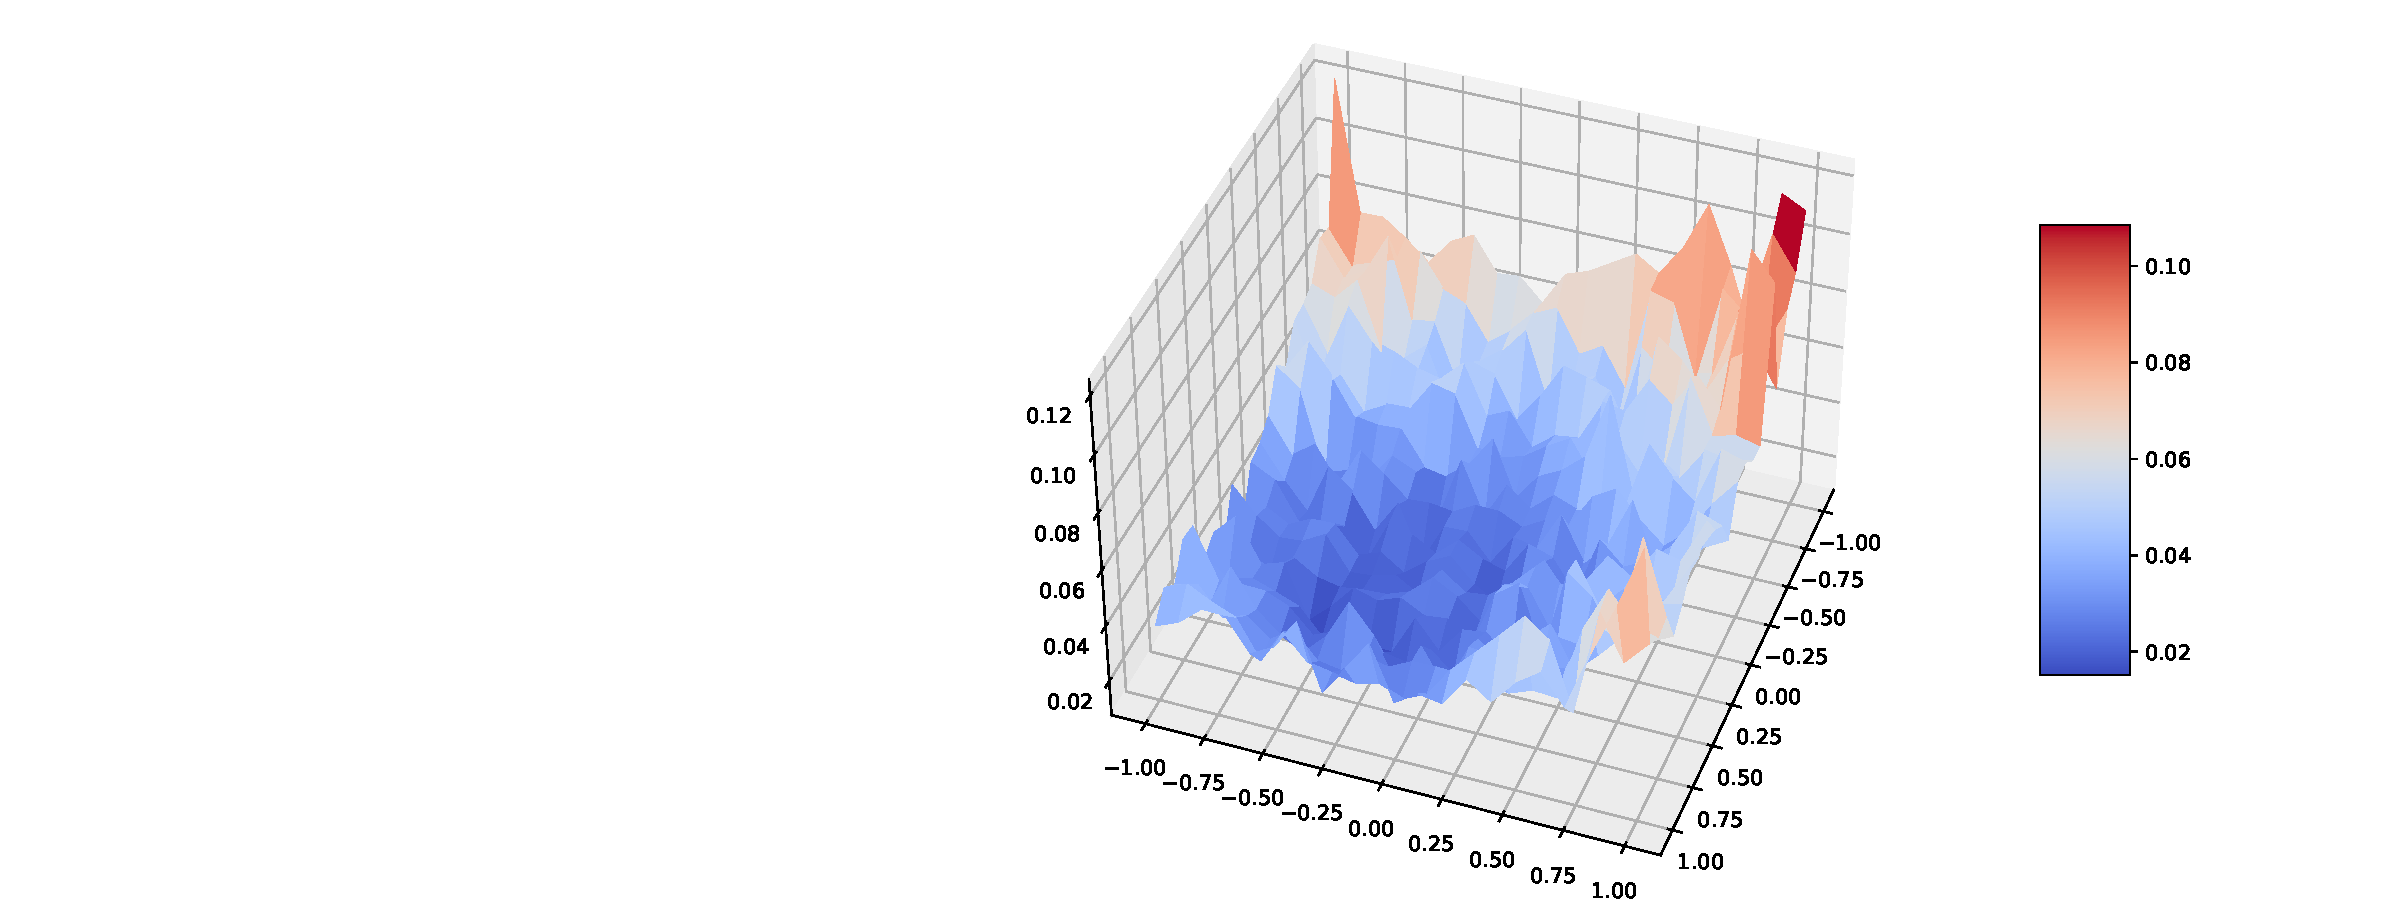
\includegraphics[width=2\textwidth]{img/Ls_16.pdf}}
  \caption{Loss function landscape}
  \label{fig:base_loss}
\end{figure}

\begin{figure}[!htbp]
  \hspace*{-11.5cm}
  \subfloat{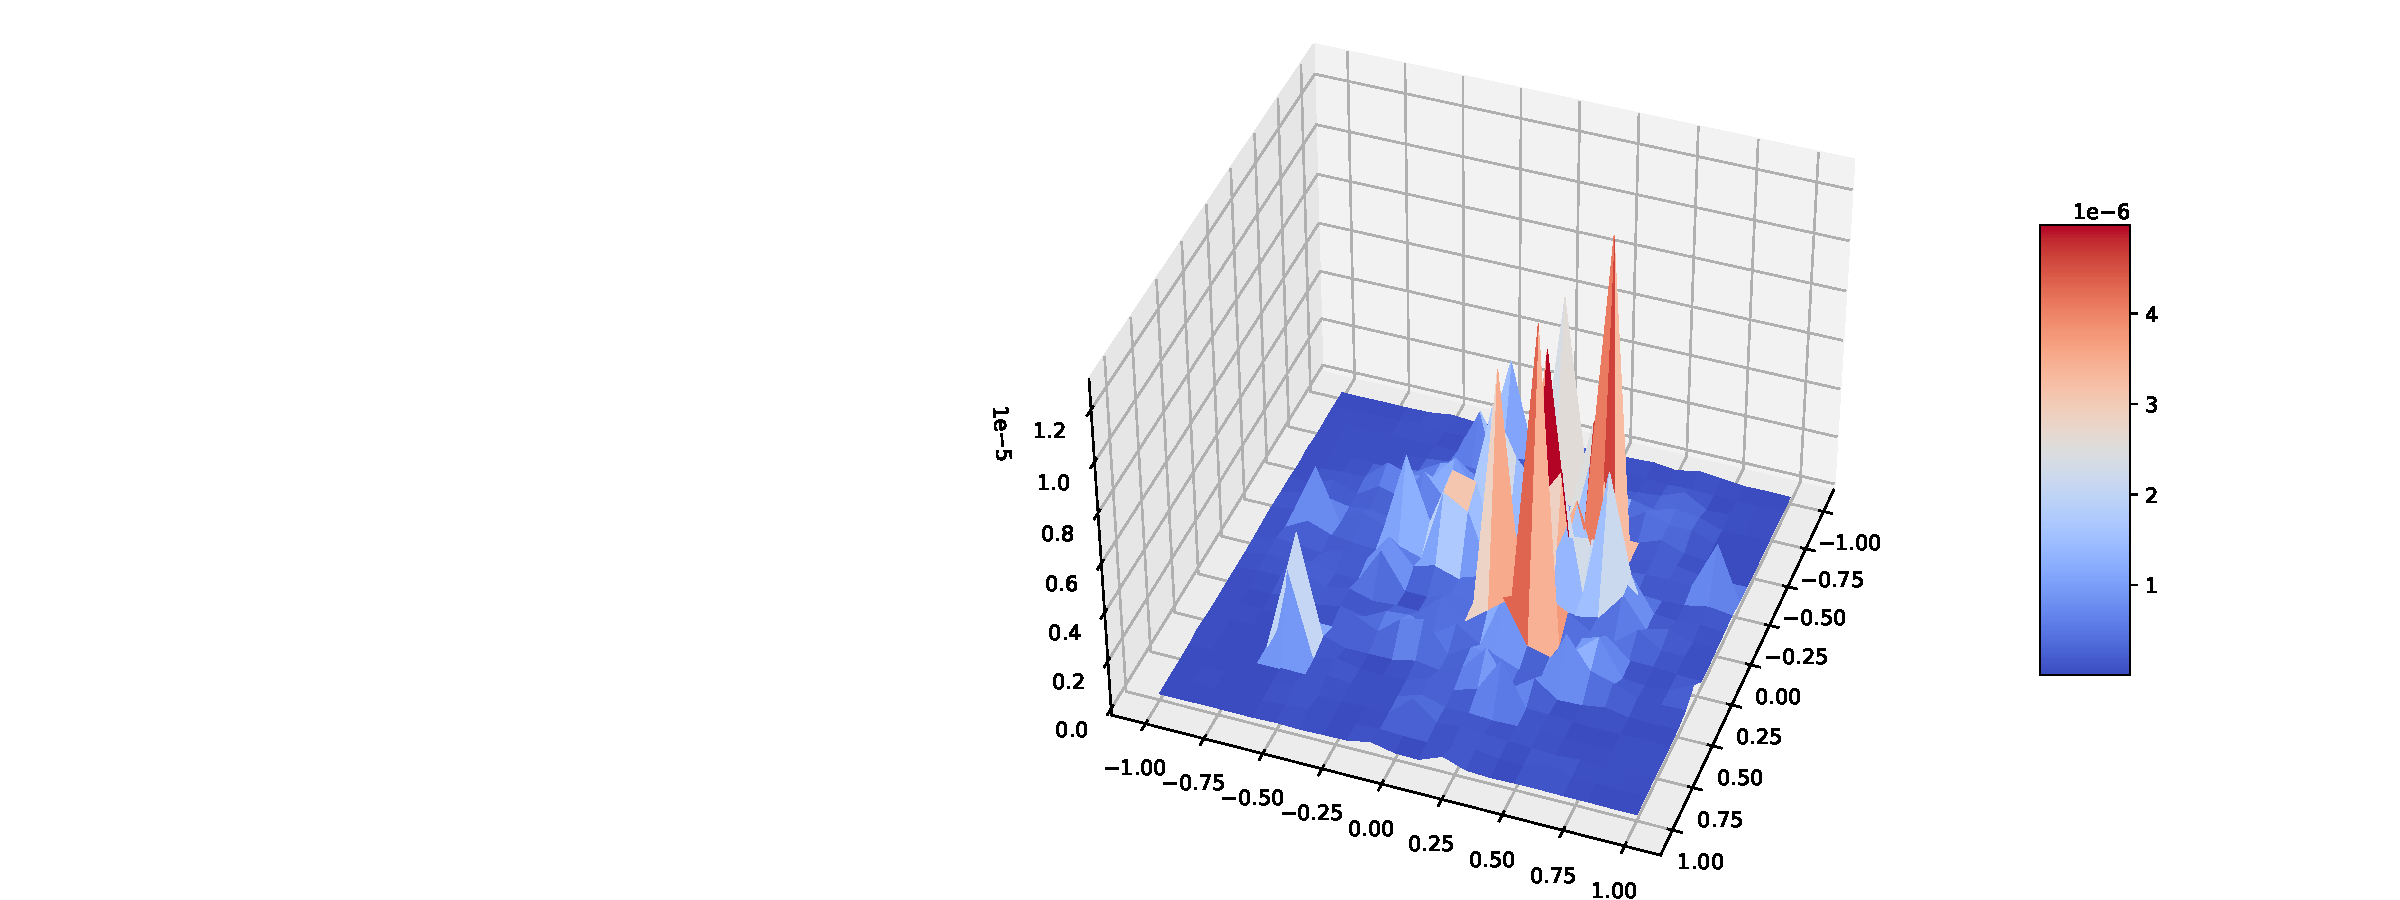
\includegraphics[width=2\textwidth]{img/Ld_10.pdf}}
  \caption{Loss function difference $(\mathcal{L}_{k} - \mathcal{L}_{k-1})^2$ landscape}
  \label{fig:base_loss_diff}
\end{figure}

\subsection{Visualizing delta-function}

Now we dig deeper and visualize our $\Delta_k$ function to clearly understand the difference in the loss function when
moving from a model trained on $k-1$ samples to one trained on $k$ samples. To do this we sample a bunch of random gaussian
vectors (all components are normally distributed) and calculate a
math expectation of modulus of the loss function difference.
Directly computing this expectation over the entire distribution of random directions $\mathbf{d}$
is impossible, so we employ a Monte Carlo approximation: using Monte-Carlo method (we take the mean value of loss function
on sampled gaussian shifted points):

$$\Delta_k = \mathbb{E}_{p(\bw)} \left( \mathcal{L}_{k}(\bw) - \mathcal{L}_{k-1}(\bw) \right)^2 \approx
  \frac{1}{k} \sum_{t=1}^{k} \left( \mathcal{L}_k(\mathbf{w}^* + \mathbf{d}_t) - \mathcal{L}_{k-1}(\mathbf{w}^* + \mathbf{d}_t) \right)^2$$

where $\mathbf{d}_t \sim \mathcal{N}(0,I_d)$ are $K$ random gaussian samples drawn from a multivariate normal distribution
with zero mean and identity covariance from a subspace of rank $d$. Specifically, we proceed as follows:

\begin{enumerate}
  \item \textbf{Sampling Directions.} Generate $K$ independent directions $\mathbf{d}_1, \dots, \mathbf{d}_M$
        from $\mathcal{N}(0,I_d)$.
  \item \textbf{Loss Evaluation.} For each direction $\mathbf{d}_t$, evaluate the loss at
        $\mathbf{w}^* + \mathbf{d}_t$ and
        $$\left( \mathcal{L}_{k}(\bw) - \mathcal{L}_{k-1}(\bw) \right)^2 $$
  \item \textbf{Averaging.} Average these values values over $k = 1, \dots, K$ to approximate $\Delta_k$.
\end{enumerate}

By increasing $K$, we obtain a more reliable estimate of the expected difference in loss landscapes.
This Monte Carlo approach is straightforward to implement and does not require explicit knowledge of the underlying loss
function's distribution.

The $\Delta$-function generally decreases as $N$ increases, suggesting that the landscape differences between neighbouring
sizes become smaller.
Beyond a certain point, $\Delta$-values are nearly negligible, indicating that adding more data has minimal impact on
the local landscape in these directions.


\noindent
\textbf{Conclusion from Preliminary Experiments.}
These initial experiments demonstrate that the loss landscape becomes progressively more stable with increasing $N$.
However, the directions used here are either random. This motivates a more rigorous approach in the \emph{main experiment}
below, where we focus specifically on the most critical directions of curvature --- those corresponding to the top
eigenvalues of the Hessian.

\subsection{Main Experiment: Projection onto Dominant Hessian Eigenvectors}

\paragraph{Rationale}
From prior work \cite{sagun2018empirical}, we know that only a few Hessian eigenvectors (those associated with the largest
eigenvalues) tend to capture the most significant curvature directions. By projecting onto these principal directions,
we can more precisely measure how the landscape the loss surface changes as $k$ increases.

\paragraph{Procedure}
\begin{enumerate}
  \item \textbf{Hessian approximation.} For each trained model, approximate
        the Hessian $\mathbf{H}$ or its dominant eigenvalues/eigenvectors. Techniques ???
  \item \textbf{Eigen-decomposition.} Identify the top $d$ eigenvectors $\{\mathbf{e}_1, \dots, \mathbf{e}_d\}$ with the
        largest eigenvalues.
  \item \textbf{Subspace exploration.} For each model, calculate a $\Delta$ fuction via the same way as in the second
        experiment (using Monte-Carlo) and appy visualization/.
\end{enumerate}

\paragraph{Goal and Expected Outcome}
\begin{itemize}
  \item \textbf{Refined understanding.} By focusing on the directions of largest curvature, we expect a clearer
        measure of how the landscape of the loss surface changes with additional data.
  \item \textbf{Identifying the threshold.} This approach should yield a more accurate estimate of the point at which the
        landscape effectively stabilizes, thus helping to pinpoint a minimum viable dataset size.
  \item \textbf{Connect with theoretical results.} By applying experiments we check our calculations above on the reality.
\end{itemize}





\begin{figure}[!htbp]
  \hspace*{-0.7cm}
  \subfloat{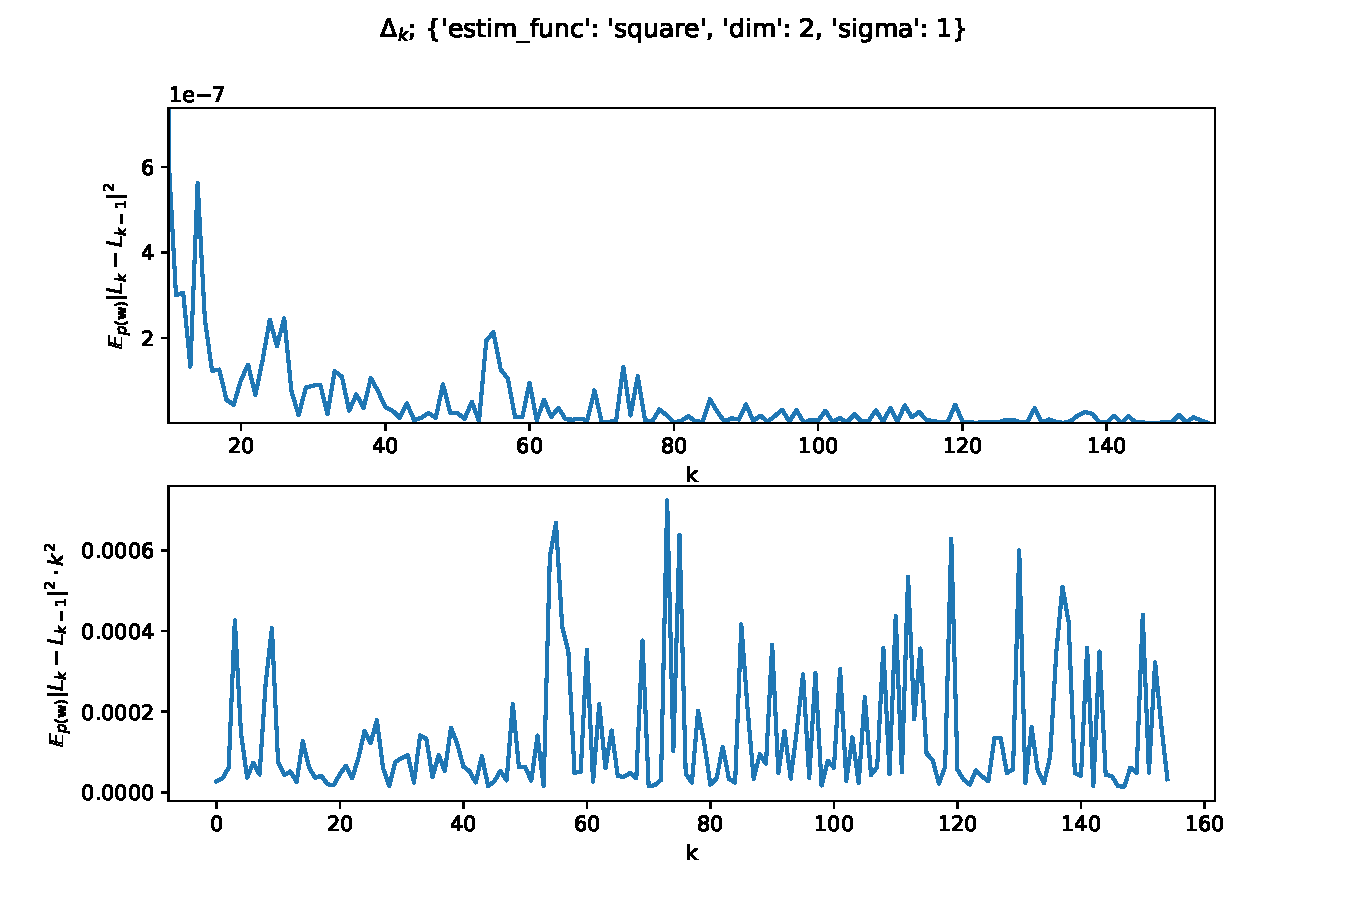
\includegraphics[width=1.15\textwidth]{img/D_32.pdf}}\\
  \caption{$\Delta$-function visualization. `Sigma` parameter refers to the variance of sampled gaussian vectors, `dim' 
  refers to the rank of the subspace.}
  \label{fig:base_delta}
\end{figure}



\section{Discussion}\label{sec:disc}

TADAAA!

\section{Conclusion}\label{sec:concl}

TADAAA!


%%%%%%%%%%%%%%%%%%%%%%%%%%%%%%%%%%%%%%%%%%%%%%%%%%%%%%%%%%%%

\bibliographystyle{unsrtnat}
\bibliography{references}

%%%%%%%%%%%%%%%%%%%%%%%%%%%%%%%%%%%%%%%%%%%%%%%%%%%%%%%%%%%%

\newpage
\appendix
\section{Appendix / supplemental material}\label{app}

\subsection{Additional experiments / Proofs of Theorems}\label{app:exp}

TADAAA!

\end{document}
